The data that we used to make this application was downloaded from the \ac{ECDC} which is an \ac{EU} agency aimed at strengthening Europe's defenses against infectious diseases.
As we can read in the \ac{ECDC} website \cite{dataDownload}, they are providing an overview of the progress in the rollout of COVID-19 vaccines in adults across \ac{EU} countries.
\begin{figure}[h]
\centering % para centralizarmos a figura

\includegraphics[width=3cm]{images/ecdc.png} 

\caption{ECDC logo}
\label{figura:qualquernome}
\end{figure}

The data is collected through The European Surveillance System (TESSy) and they publish the updated data, every week on Thursdays. In Portugal, the entity responsible to send the data is the Ministry of Health.

\subsection{Structure of the data}
The dataset that we downloaded, in format CSV, has the following columns:

\begin{itemize}
    \item \textbf{YearWeekISO} - The date information. Here we can see the number of week and year on the data;
    \item \textbf{FirstDose} - Number of first dose vaccine administered to individuals during the reporting week;
    \item \textbf{FirstDoseRefused} - Number of individuals refusing the first vaccine dose;
    \item \textbf{SecondDose} - Number of second dose vaccine administered to individuals during the reporting week;
    \item \textbf{UnknownDose} - Number of doses administered during the reporting week where the type of dose was not specified;
    \item \textbf{NumberDosesReceived} - Number of vaccine doses distributed by the manufacturers to the country during the reporting week;
    \item \textbf{Region} - Certain Region of the Reporting Country;
    \item \textbf{Population} - Age-specific population for the country (unfortunately, in Portugal, this hasn't been exactly right, it only has the total population of Portugal);
    \item \textbf{ReportingCountry} - The country that is providing the information;
    \item \textbf{TargetGroup} - Target group for vaccination;
    \item \textbf{Vaccine} - Name of vaccine;
    \item \textbf{Denominator} - Population denominators for target groups.

We will show next, a little example of the dataset already filtered for Portugal.

\end{itemize}

\begin{figure}[h]
\centering % para centralizarmos a figura
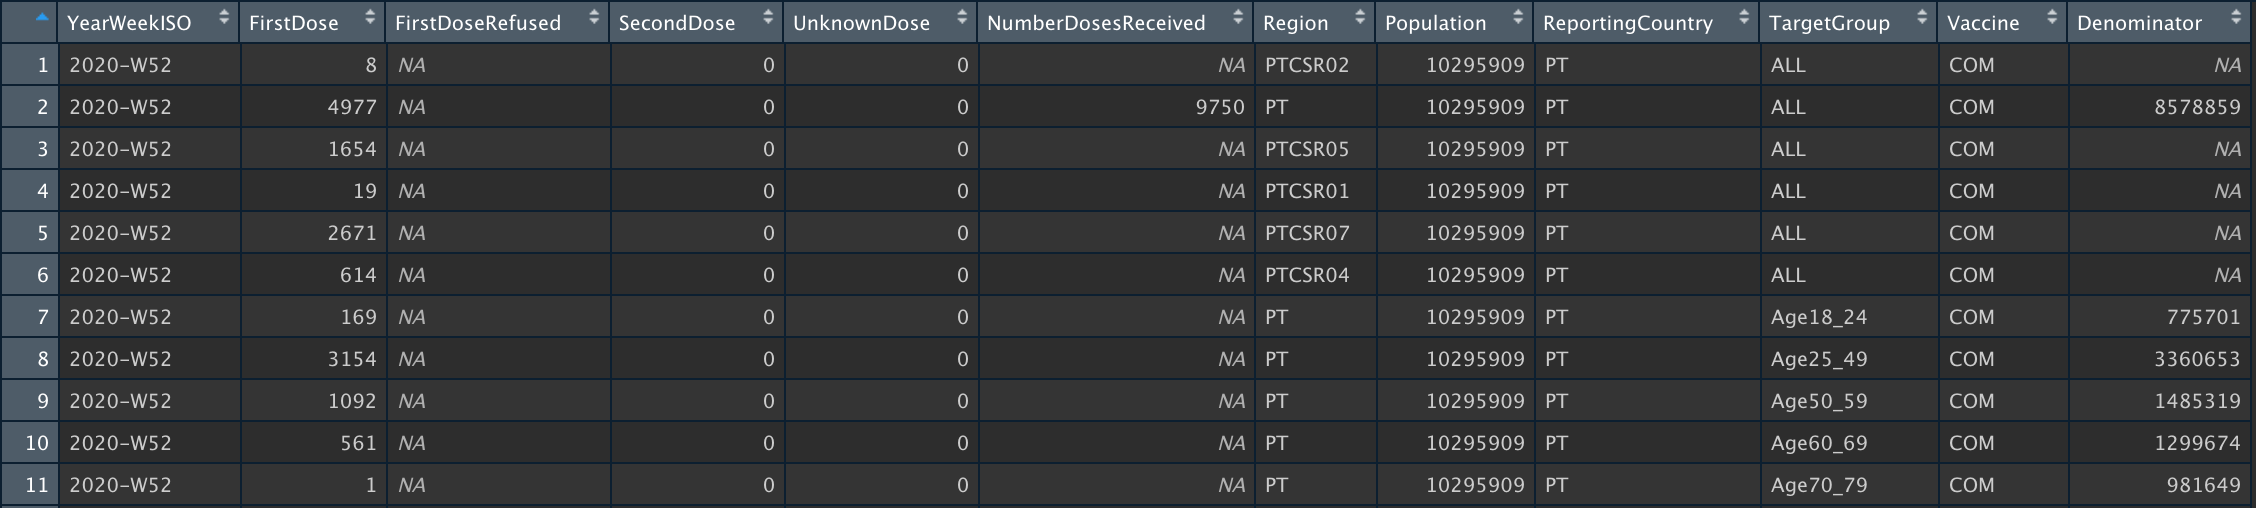
\includegraphics[width=15cm]{images/dataset.png} 

\caption{Excerpt from the dataset }
\label{figura:qualquernome}
\end{figure}

\subsubsection{Notes about Portugal's data}

There are some aspects about the Portugal's data that we notice throughout the development of this application. We will listed them next:
\begin{itemize}
    \item Continuar aqui!! Ha algumas cenas interessantes que deveremos por aqui tipo:
    o que significam as siglas de Region.
    \item Siglas das vacinas
    \item e mais cenas que encontramos durante a realização desta cena
\end{itemize}